\section{Evaluation}
\label{sec:evaluation}
% measured-evidence-begin: long-history-evaluation
% EVIDENCE-H100-LONG-HISTORY; EVIDENCE-H100-DEADLINE-AUDIT

We evaluate whether retaining long histories in host memory increases the periodic work that fits within a realistic GPU KV budget, and whether advance restoration reduces the resulting service delay.
The measurements compare three systems at two offered loads, using real model execution after long-history initialization.
Each of the six points is measured once.
We report completion counts, latency distributions, physical KV allocation, and transfer costs over the observed window.

\subsection{Methodology}
\label{sec:methodology}

\paragraph{Platform and workload.}
We run MiniCPM-o 4.5 in BF16 on one NVIDIA H100 80GB HBM3 GPU, using vLLM 0.23, PyTorch 2.11, and Transformers 4.57.6.
The host exposes 16 logical CPUs on an AMD EPYC 7R13 and approximately 249.69\,GiB of RAM; these host details were recorded in a same-machine post-run probe.
The GPU KV pool is 48\,GiB, reserving the rest of device memory for weights and execution; the managed systems have an 80\,GiB host backing pool.
A physical KV block holds 16 positions and occupies 2.25\,MiB.
Each session receives two seconds of recorded LibriSpeech dev-clean audio per update and generates eight text tokens, with a two-second period.
The measured path processes recorded speech and generates text.

Each session begins with an actual model prefill of 30,000 synthetic text tokens, constructed reproducibly with a unique prefix for each session.
For managed systems, setup proceeds session by session, backing and safely evicting state before initializing the next session.
The resident system initializes only admitted sessions.
Prefill completes before the common source clock begins and its output is excluded from service measurements.
Retained context then grows through real audio processing and text generation, reaching 30,673 positions within the common 32,768-position backend limit.
The initial text history accelerates the capacity experiment; it is not a natural long conversation.

We offer either 12 or 14 sessions with staggered source clocks, distinct recording offsets, and input seed 11.
Each session supplies 24 seconds of audio, yielding 12 updates.
The primary measurement window excludes the first six seconds on the common source clock, leaving ten updates per admitted session.
We additionally report the full input sequence, including startup, to expose effects hidden by that exclusion.
Every point starts a fresh worker with eager execution, a 4,096-token batch limit, and at most 16 scheduled sequences.
Sampling uses temperature zero with EOS stopping disabled, enforcing the common eight-token budget.
GPU activity profiling and intrusive copy validation are disabled for these measurements.

\paragraph{Compared systems.}
\emph{Full residency} keeps all retained history on the GPU, uses naturally staggered phases, and admits 11 sessions.
This limit fits the history reached in the measured window; it is not a reservation for all sessions reaching the backend's maximum context.
\emph{On-demand restoration} uses the same host backing, partial eviction, assigned phases, and copy implementation as \systemname, initiating restoration when preprocessing finishes and current computation needs its history.
\emph{\systemname} initiates restoration through an independent timer before the next planned tick, with a configured lead of 350\,ms.
Both managed systems use four phase slots and the same fixed admission limits of 12 or 14 for the respective offered loads.
Their per-session eviction ceilings are 256 blocks at 12 sessions and 640 blocks at 14 sessions.
These matched fixed cohorts exercise residency management and restoration timing; they do not measure the admission planner's ability to select a feasible maximum-context population.
The different eviction ceilings also mean the two load points are configured operating points, not a sweep with every policy parameter held constant.

\paragraph{Completion and accounting.}
Let $r(i,k)$ be an update's planned tick, $a(i,k)$ its original source-ready time, and $c(i,k)$ the associated generation completion.
The primary deadline is $r(i,k)+T$, and periodic completion latency is $c(i,k)-r(i,k)$.
We also report $c(i,k)-a(i,k)$, which includes phase-alignment waiting.
Delayed submission never moves an update's deadline.
A supplementary, post-hoc sensitivity counts completions by $a(i,k)+T$ to compare all systems against the same input clock.
This stricter source-clock criterion is distinct from the primary planned-tick objective.
Rejected demand stays in the offered-work denominator; unfinished admitted work is counted separately.
Completion comes from the engine's fixed-budget generation event, not an RPC return or buffered output.

GPU occupancy counts allocated physical blocks, including complete restoration destinations while copies are in flight.
Host backing counts valid cached copies and may include reclaimable copies; it is distinct from the reserved host pool.
We count submitted physical transfer bytes, without interpreting CPU copy-control intervals as pure DMA time.
Separate correctness checks verify exact KV bytes across multilayer, noncontiguous D2H/H2D copies, unchanged unrelated destinations, and restored logical block mappings.
These checks are excluded from performance runs.

\subsection{Capacity and Service Cost}
\label{sec:eval-main}
\label{sec:eval-capacity-bound}

\begin{table}[t]
\centering
\caption{Primary measurement window on MiniCPM-o 4.5. All admitted updates complete on time under the planned-tick deadline; none remain unfinished. Latencies are p95 in milliseconds.}
\label{tab:measured-capacity}
\begin{tabular}{@{}llrrrr@{}}
\toprule
Offered & System & Admit & On time & Tick & Source \\
\midrule
12 & Resident & 11 & 110 & 289 & 289 \\
   & On-demand & 12 & 120 & 407 & 1683 \\
   & \systemname & 12 & 120 & 283 & 1626 \\
\midrule
14 & Resident & 11 & 110 & 282 & 282 \\
   & On-demand & 14 & 140 & 1380 & 2488 \\
   & \systemname & 14 & 140 & 573 & 1925 \\
\bottomrule
\end{tabular}
\end{table}

At 14 offered sessions, both managed systems admit and complete work for all 14, compared with 11 under full residency (Table~\ref{tab:measured-capacity}).
This is a 27.3\% increase in served sessions and on-time updates in the primary window, from 110 to 140 updates, with no unfinished work.
The resident baseline remains responsive for its admitted sessions and rejects the other three.
The additional admitted sessions complete their periodic work while the protected resident baseline continues serving its admitted sessions promptly.

The capacity gain uses most of the available GPU KV pool.
Peak physical allocation is 46.31\,GiB for residency, 47.45\,GiB for on-demand restoration, and 47.50\,GiB for \systemname.
At the same high-load point, both managed systems retain up to 62.85\,GiB of valid host backing within their 80\,GiB pools.
The managed systems therefore serve aggregate retained state larger than the GPU KV budget, while using almost all of the available pool.

\paragraph{Restoration timing.}
\label{sec:eval-latency}
At 14 admitted sessions, advance restoration lowers periodic p95 completion latency from 1,379.8 to 572.9\,ms, a 58.5\% reduction relative to the matched on-demand system.
Including source-clock alignment, p95 latency falls from 2,487.6 to 1,924.5\,ms, a 22.6\% reduction.
The p95 interval from preprocessing completion to engine enqueue falls from 726.3 to 167.4\,ms, or 77.0\%.
This interval includes history readiness and control handoff; it is not a measurement of DMA alone.
The shared phase and eviction settings isolate the change in restoration trigger.

At 12 offered sessions, \systemname completes 120 on-time updates versus 110 for residency, and its periodic p95 latency is 283.4\,ms versus 406.7\,ms for on-demand restoration.
Source-clock p95 is 1,626.0 versus 1,683.2\,ms, showing that phase alignment can dominate user-visible delay even when restoration waiting is small.
Full residency has lower source-clock latency at both loads while serving fewer sessions, exposing the capacity--latency tradeoff.

\begin{figure*}[t]
\centering
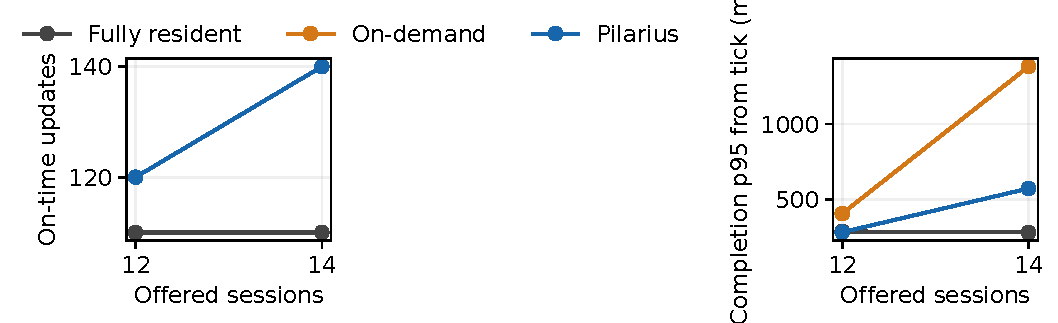
\includegraphics[width=\linewidth]{figures/evaluation-capacity.pdf}
\caption{Capacity and periodic completion latency in the primary measurement window. Each marker is one run; lines connect configured operating points. Both managed systems complete more work than residency, while advance restoration reduces the matched on-demand delay.}
\Description{Two load points compare on-time updates and completion latency across residency, on-demand restoration, and Pilarius.}
\label{fig:capacity-results}
\end{figure*}

\subsection{Startup and Deadline Sensitivity}
\label{sec:eval-deadlines}

\begin{figure*}[t]
\centering
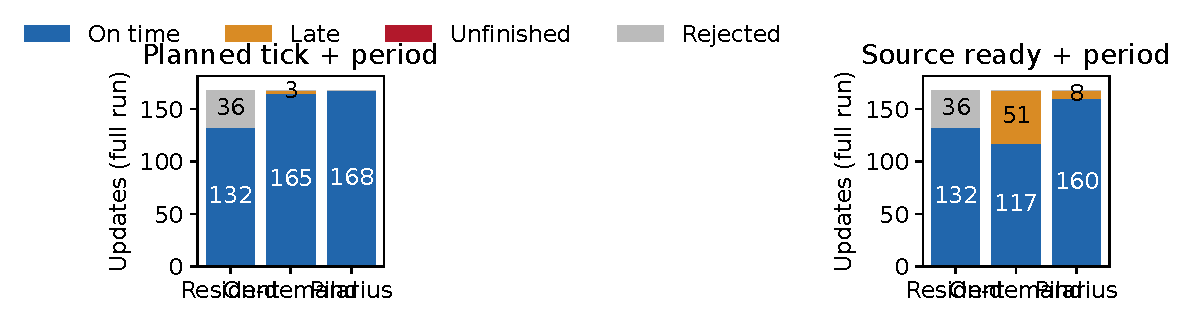
\includegraphics[width=\linewidth]{figures/evaluation-deadlines.pdf}
\caption{All 168 offered updates at the 14-session point, including startup. Left: the primary planned-tick deadline. Right: a supplementary source-ready-plus-period criterion that includes alignment waiting. Rejected demand is shown separately from late admitted work.}
\Description{Stacked bars distinguish on-time, late, unfinished, and rejected updates under planned-tick and source-clock deadlines.}
\label{fig:deadline-sensitivity}
\end{figure*}

Across the full 12-update sequence at 14 offered sessions, residency completes 132 updates on time and rejects 36 updates' worth of demand.
On-demand restoration completes all 168 updates but misses three planned-tick deadlines; \systemname completes all 168 without a planned-tick miss.
The zero-miss observation for on-demand restoration in Table~\ref{tab:measured-capacity} therefore applies only after excluding the first six seconds.

Figure~\ref{fig:deadline-sensitivity} also includes phase waiting through the source-clock criterion.
Residency completes 132 updates within two seconds of their source readiness, on-demand restoration completes 117, and \systemname completes 160.
The latter corresponds to 21.2\% more timely work than residency and 36.8\% more than on-demand restoration under this supplementary criterion.
The managed systems have 51 and eight late updates, respectively, and no unfinished work.
Their full-run source-clock p95 latencies are 2,755.0 and 1,983.1\,ms.
At 12 offered sessions, all admitted updates satisfy both deadline definitions in the full run.

\subsection{Coverage and Cross-Model Interpretation}
\label{sec:eval-coverage}

The measurements cover two fixed cohorts with long initial histories, one workload configuration, and one run per point.
They establish the observed capacity and restoration-delay tradeoff over 24 seconds of input per session.
Run-to-run variability, dynamic arrivals, independent phase assignment, and longer-term operation remain outside this evaluation.
The initial histories contain synthetic text, and the measured output is text; conversation quality and native speech output require their own workloads.

A second model has executed through the shared management path in separate integration and calibration runs.
The cross-model and cross-hardware tables in Section~\ref{sec:capacity-problem} extend the resource analysis using public model geometry and explicit efficiency assumptions.
Their entries are analytical estimates; the capacity and latency results above come from the measured configuration.
